\section{Evaluation}
\label{evaluation}
Evaluation section is divided into four types of experiments: First, we are showing the effect of batching and batching plus prefetching for each application. Second, we are comparing our applications with the same application with hand-tuned optimizations published in different papers. By doing this we are showing that automatic optimizations can work as good as hand-tuned optimizations. Third, we are running the applications with different number of cores to show that the applications are scaling linearly with the number of cores. Fourth, we are comparing the throughput by changing the batch size and table size for L2FWD application to show the relation among batch size, table size, and throughput. With this experiment we are also making sure that our model is working the same way we are expecting.

\subsection{Evaluation Setup}
\textbf{Server Specifications:} We are using Dell Poweredge R430 Rack Server, based on Haswell architecture. This server has two sockets occupied with Intel Xeon E5-2640 
v3\cite{xeon} processor. Each processor has 8 physical and each core is capable of running at 2.60 GHz. Cores on a socket share 20 MB cache. Sockets are connected with 2 QPIs(Quick Path Interconnect), each capable of 8 GT/s. Two dual port NICs,1 Intel x520 and 1 Intel x540, are connected to Socket 0 through PCIe 2.0 and each port can work at 10Gbps. Total main memory available is 64 GB, spread across two sockets in a NUMA fashion.
\\
\\
\textbf{Software:} Our servers are running Ubuntu 14.04 LTS operating system with 4.4.0-59 Linux kernel version. We are using DPDK version 16.07 with IXGBE poll mode driver to
interact with the underlying NICs. 
\\
\\
\textbf{Traffic Generator:} We are using same hardware and software on both the servers and Pktgen-DPDK\cite{pktgen} version 3.1.0 to generate different kind of packets for different applications used in the experiments. Pktgen-DPDK\cite{pktgen} can generate the 64 bytes packet size traffic at line rate i.e 14.8 Mpps for 10 Gbps port. We are able to generate traffic at 59 Mpps for four ports with 64 bytes packet size. We have extended Pktgen-DPDK\cite{pktgen} to put random source and destination address depending on the application.
\\
\\
\textbf{Applications:} In this part we are specifying the applications we are using for different experiments. We have written applications in P4\cite{Bosshart:2014:PPP:2656877.2656890} and extended P4C\cite{Laki:2016:HSP:2934872.2959080} compiler to generate code with the above mentioned optimizations. P4C\cite{Laki:2016:HSP:2934872.2959080} is generating DPDK\cite{DPDK} based applications which are later compiled with gcc to get the target binary. We are using similar application as used in \cite{189006} for comparing our results with their CPU based implementation. 
\begin{enumerate}
 \item \textbf{Layer 2 Switch:} In this application we are using two hash tables to store the mapping between SMAC/DMAC and value. Each packet is going through two lookup stages, one for SMAC and one for DMAC. We are putting 16 Million entries in the table for the experiments, unless otherwise specified for some experiment. We are using Intel DPDK's implementation for various hash table operations.
\item \textbf{IPV4 Forwarding:} In this application we are performing LPM lookup on destination IP address to get the forwarding port. We are using Intel DPDK's implementation for LPM related operations for IPv4 Forwarding and IPv6 Forwarding application. We are populating the forwarding table with 527,961 prefixed used by \cite{189006}. 
\item \textbf{IPv6 Forwarding:} We are preforming one lookup on destination address to find the egress port. We are populating the DPDK LPM table with random 200,000 entries with the length between 48 to 64, as done in \cite{189006}. From the Pktgen we are generating the packets with destination address randomly picked from these 200,000 entries. Minimum packet size for this application is 78 bytes and not 64 bytes.
\item \textbf{Named Data networking:} We are using hash table for lookups implemented by DPDK. We are using algorithm and URL dataset from \cite{DBLP:conf/globecom/ZhangWYLL13}. From Pktgen we are generating packet by randomly putting the URLs from used dataset. We are using 32 bytes URLs in the packet headers as done in \cite{189006}.
\item \textbf{l2fwd-crypto Application:} All other applications are lookup based and we want to see the effect of batching \& prefetching on other kind of applications too. So, we have included this application in the experiments. We are using L2Fwd-Crypto\cite{l2crypto} from DPDK examples given in DPDK repository. The application performs encryption and decryption based on the input parameters and then it forwards the packet on Layer 2 with static port mapping. 
\end{enumerate}

\subsection{Effect of batching and prefetching}
\label{batchingandprefetching}
\begin{figure}[ht]
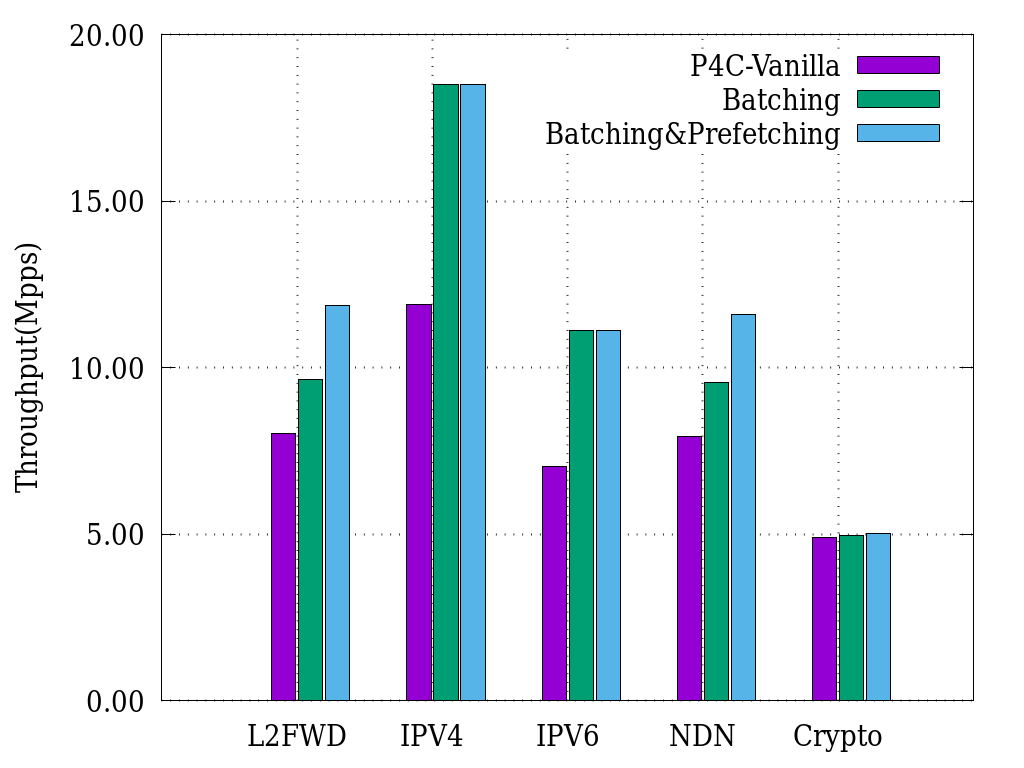
\includegraphics[width = \linewidth]{Figures/effectofbatching.png}
\caption{Effect of batching and prefetching}
\label{batchingandprefetchingfigure}
\end{figure}
In P4C\cite{Laki:2016:HSP:2934872.2959080}, authors are not using batching and prefetching for the applications. We are adding batching and prefetching for all the applications and in Figure \ref{batchingandprefetchingfigure} we are showing the effect of these optimizations for different applications. We are using 32 as batch size for all the applications in all the experiments unless specified otherwise. L2Fwd and NDN are using hash lookup and DPDK code is written in such a way that we are able to prefetch the bucket where the key is present. On the other hand, we don't have much opportunity to use prefetches for LPM lookup based applications. For L2Fwd, batching improves the performance by 20\% and prefetching, used with batching, again improves the performance by 23\%. Similarly for NDN, batching alone improves the performance by 20\% and after adding prefetching there is an additional performance gain of 21 \%. After applying batching and prefetching to IPv4 and IPv6 there is a performance gain of 55\% \& 57\% respectively.
\\
\\
\textbf{Conclusion:} As we can see that batching can be used for almost all the applications without thinking much. The only challenge is to come up with the optimal batch size. Section \ref{optimalbatchsize} can be used to find the optimal batch size. Prefetch on the other hand surely improves the performance but can't be used in every application and should be used with precaution as it might pollute the cache which might result in performance loss.

\subsection{Comparison with hand-tuned applications}
\label{comparisonexperiment}
\begin{figure}[ht]
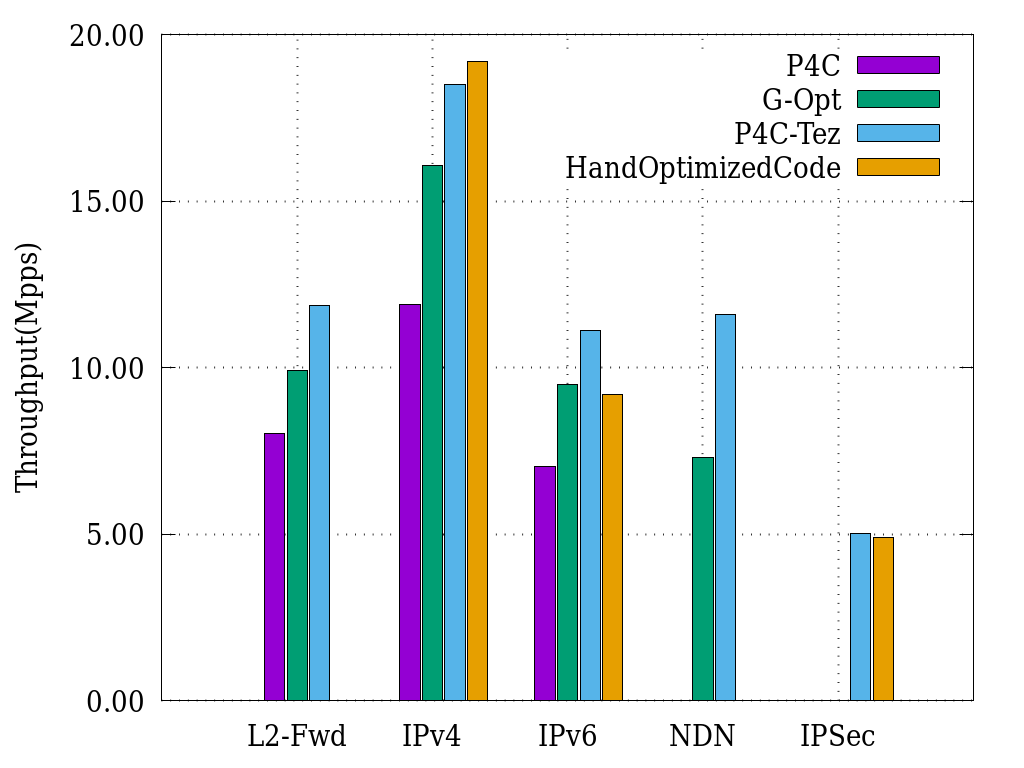
\includegraphics[width = \linewidth]{Figures/comparison.png}
\caption{Comparison with other hand-tuned applications}
\label{comparisonfigure}
\end{figure}
In Figure \ref{comparisonfigure}, we are comparing our automatic generated code with comparable hand-tuned code and vanilla P4C\cite{Laki:2016:HSP:2934872.2959080}. We are making sure that number of lookups and number of entries in the table(s) are same in all the cases so that we can show the comparison among applications. For some of the applications it is not possible to compare our application with the hand-tunes application and we have omitted the bar from the graph for such applications.
\\
\textbf{Comparison with vanilla P4C\cite{Laki:2016:HSP:2934872.2959080}:} This is the most suitable comparison because we are using the same applications and same flow in our applications. There is 48\%, 55\%, 57\%, and 46\% improvement for L2Fwd, IPv4, IPv6, and NDN application respectively. In the applications, they are not exploiting batching \& prefetching and just with these optimizations there is a huge improvement.
\\
\textbf{Comparison with G-Opt\cite{189006}:} There is 20\%, 15\%, 17\%, 59\% improvement for L2Fwd, IPv4, IPv6, and NDN application respectively. They are using both batching and prefetching, and there main aim was to make the results comparable to GPU. The difference is due to the batch size, they are not using the optimal batch size and we can see the performance gain by using the optimal batching size in Figure \ref{tablesize}.
\\
\textbf{Comparison with DPDK\cite{DPDK}:} For IPv4 DPDK is performing 4\% better than our code and for IPv6 we have a performance gain of 20\%. The result for IPv6 doesn't include the improvement we are gaining by TRIE compression, that will be reported later in this section. 
\\
\\
\textbf{Conclusion:} By using the optimal batch size and right prefetch distance we are performing almost equal or better than other hand-tuned optimized code. Even if the results are equal we can say that our approach is better than hand-tuned one, because it is one-time efforts and can be used for wide variety of applications. Results in figure \ref{comparisonfigure} are for one core and we will show in Section \ref{scalability} that our applications are scaling linearly with the number of cores.


\subsection{Scalability}
\label{scalability}
\begin{figure}[ht]
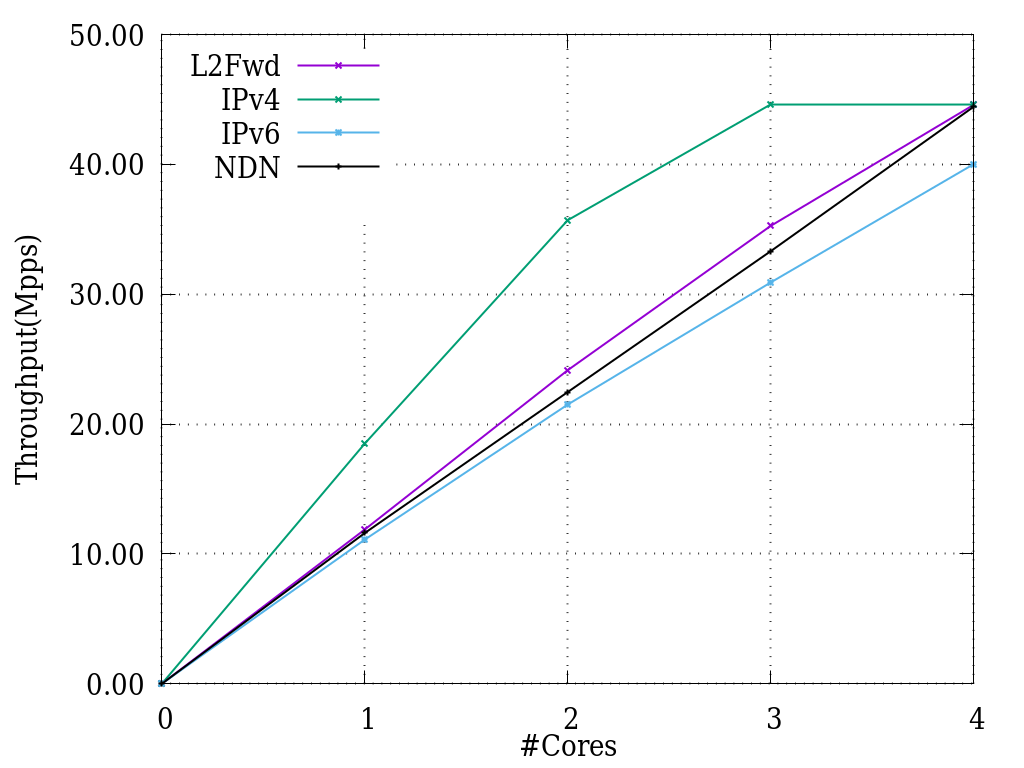
\includegraphics[width = \linewidth]{Figures/cores.png}
\caption{Number of Cores vs Throughput}
\label{cores}
\end{figure}
In Figure \ref{cores}, we are showing that our applications are scaling with the number of cores. With 4 cores we saturating 4 ports(4 x 10 Gbps) when the packet size is 64 bytes.
The theoretical limit for 4 NICs is 59 Mpps but we are getting 44 Mpps as shown in the graph. PCIe is the bottleneck in this case and not the applications. When one NIC is sending and receiving at both the port then it can reach up 22 Mpps and not theoretical maximum 29 Mpps. \cite{Zhou:2013:SHP:2535372.2535379} has also mentioned about this bottleneck in the paper.

There is not much to talk about L2Fwd and NDN application, these applications are scaling linearly. IPv6 is not reaching upto 44 Mpps with 4 cores and that is because of large packet size for IPv6. We are using 64 bytes packets for other applications but Pktgen-DPDK is generating 78 bytes packets for IPv6. Hence IPv6 application is also saturating the ports with 4 cores. The other interesting part of the graph is the IPv4 line, till 2 cores the application is scaling linearly and after that it is coming down. There is no more available bandwidth for the application and it is saturating it with three cores. 
\\
\textbf{Conclusion:}We can say two things about the result of this experiment. First, applications are scaling linearly with the number of cores and second, applications are saturating four 10 Gbps ports with four cores.

\subsection{Relation between Batch Size, Table Size, and Throughput}
\label{batchvstable}
\begin{figure}[ht]
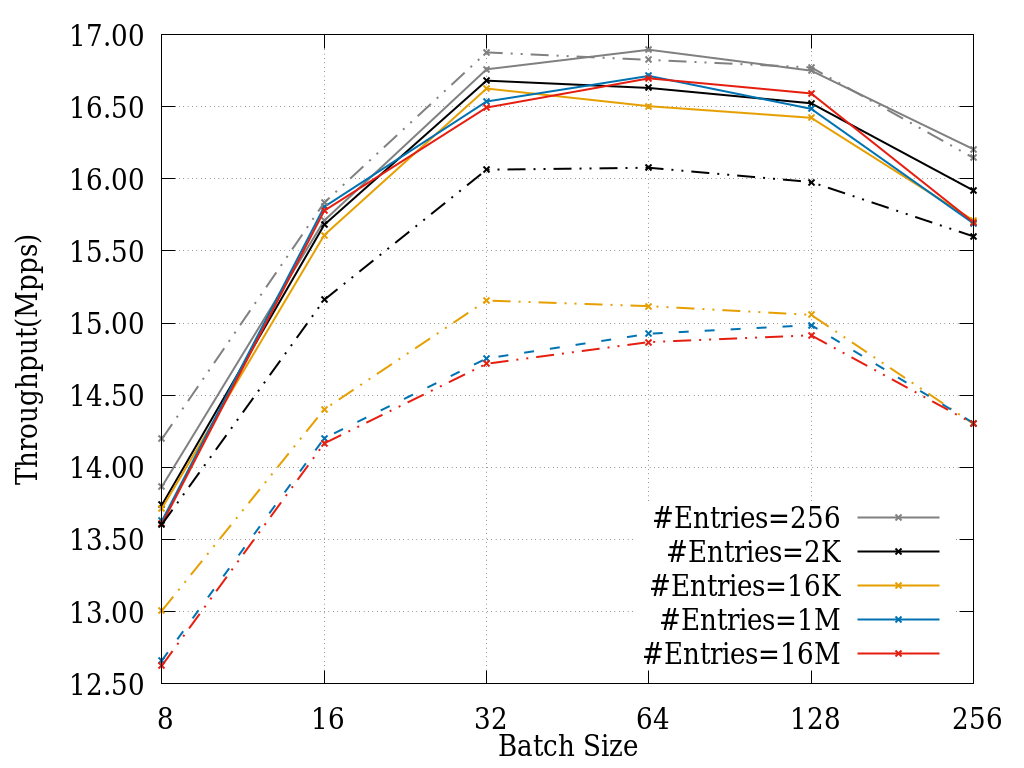
\includegraphics[width = \linewidth]{Figures/TableSizeVsbatchSize.png}
\caption{Throughput vs Batch Size}
\label{tablesize}
\end{figure}
In Figure \ref{tablesize}, we are showing the relation between throughput and batch size for different number of entries in the lookup table. We are using L2-FWD application with one lookup for this experiment. In the graph we are  

Throughput is increasing with increase in batch size till 64 and for same batch size the difference in the throughput is not much when we are varying the entries from 256 to 16 Million.
\\
\textbf{Effect of Batch Size:} Throughput is increasing with increase in batch size, the increase is sharp until the batch size reaches 32. After 32 batch size, there is a small rise in throughput when batch size is changed to 64. There is decline in throughput when batch size is increase to 128 and more. 
\\
\textbf{Effect of Table Size:} We can summarize the result in two main points. First, there should be a decline in the throughput with increase in the number of entries and throughput of the application should be more when there are less number of entries in the table. However this is not the case when we see in Figure \ref{tablesize}. In Eq \ref{compute_througput} we can see that for each packet CPU needs to do some processing and there are some memory operations associated with each packet. If the memory pressure is more the number of stall cycle will be more and the performance of the application would decrease. For larger table size, data won't be present in the cache and application must stall on it. However, we are prefetching the data even before the data is used in the application and this prefetching of data is reducing the total stall cycles as described in Eq \ref{cycles_stall}. This is the reason that the throughput of the application is stable and not varying much with increase in the number of entries in the table. 

Second, for each batch size the relative throughput of the application will be dictate by the number of entries in the table. In actual, the results are quite opposite to the expectations and this is because total stall time reduction is dependent on effective prefetch distance. One batch size may not work for different number of entries and relation between table size, batch size, and effective prefetch distance has been summarized in Section \ref{subbatching}. Let's take an example of batch size 64, the throughput of the application is more when there are 1 M and 16 M entries as compared to 2 K \& 16 K entries in the table. The data will be in L2/L3 cache for these many number of entries and due to large batch size, entries will be prefetched way before the data will be needed in the application. On the other hand for larger table sizes, larger batch size is suitable since the data will be prefected from the main memory which will take more number of cycles. For 2 K and 16 K entry table we tried to minimized the prefetch distance by using the sub-batch size of 32 and the application is performing better than the application with 1 M and 16 M entries.

\textbf{Conclusion:} 
There is an increase in throughput with increase in the batch size till 64 and then there is a decline in the throughput. In our NIC we have cache size of 40 descriptors and till 64 throughput due to IO batching is increasing but after 64 there is a decline in the throughput, hence there is a decline in the overall throughput of the application for batch size more than 64. As explained above in this section, the throughput is not declining much due to increase in the table size and we can say that batching and prefetching is playing well together and due to this the throughput is stable even if we are increasing the table size.

\subsection{TRIE Compression}
The DIR24-8\cite{Gupta98routinglookups} based Trie IPv6 lookup doesn't exploit the fact that i) many IPv6 prefixes comes from same domain and large portion of their prefixes are common. The DIR24-8 data-structure allocates a 256 entry sized tbl8 even for a single IPV6 entry. This type of over-provisioning leads to memory wastage and also increases memory accesses during lookup. ii) IPv6 prefixes coming from unique domain will be stored in a single node only regardless of its length. Despite having storage overheads compressed trie based lookup outperforms conventional lookup, based on simple trie, by avoiding very costly memory operations involved in accessing a new node. Due to compression there is a dip of 3.5\% in worst case and there is gain of 38\% in best case. Vanilla P4C throughput for IPv6 is 7.2 Mpps and after compression we are getting 8.82 Mpps, which is a performance gain of 22\%. We are getting this performance for the IPv6 entries we are using and we are not checking for best case and worst case performance gain by the compression.

\section{Related Work}
\label{relatedwork}
\textbf{CPU based packet processing:} RouteBricks\cite{dobrescu2009routebricks} is one of the first paper in this area. They exploited various components in a commodity server to achieve 35 Gbps throughput for Layer 3 Forwarding. They used both inter-server and intra-server optimizations to achieve this throughput.
\\
\textbf{Manual optimizations:} There are many papers where authors have come up with different kind of manual optimizations to show the improvement in the performance. Batching\cite{dobrescu2009routebricks, 189006, Kim:2012:PBC:2349896.2349910, Zhou:2013:SHP:2535372.2535379} has been used extensively by authors, however, these papers are determining the batch size by empirical analysis. \cite{189006, Zhou:2013:SHP:2535372.2535379} are exploiting the fact that CPU and Memory subsystem can work in parallel and memory stall can be minimized by issuing the software prefetches before actually using the data. However, it is difficult to use these manual optimizations each time we are writing a packet processing application.
\\
\textbf{Compiler optimizations:} Shangri-La \cite{Chen:2005:SAH:1065010.1065038} generates optimized binary for network processor and showing that the generated binary is working as good as hand-tuned code. \cite{Dobrescu:2010:CPM:1921151.1921154} talks about the importance of doing the optimizations in the compiler rather than hand-tuning the same thing for different applications. The main focus of paper \cite{Dobrescu:2010:CPM:1921151.1921154} is to automating the decision of breaking the application in parallel components to achieve high throughput.
Due to space constraint, we are not mentioning papers related to various kind of software based packet processors and different DSLs for writing the network applications.

\section{Conclusion}
\label{section6} 
The goal of this paper is to find the efficient batch size and right prefetch distance to use the underlying hardware efficiently and to improve the application performance. In the evaluation section, we are showing that per core performance for different applications is on par with hand-tuned optimized applications and applications are scaling with the number of cores. It saves a lot of time and efforts, and we don't need to think about the code flow for different types of applications and the possible bugs due to manual intervention. We believe that DSLs won't be very useful if we are unable to develop good compilers. The actual power of DSLs can only be realized when the compilers can generate the optimized target which is on par with hand-tuned code.